\documentclass[11pt,a4paper]{article}

\usepackage[utf8]{inputenc}
\usepackage[T1]{fontenc}
\usepackage{geometry}
\usepackage{graphicx}
\usepackage{amsmath}
\usepackage{booktabs}
\usepackage{longtable}
\usepackage{float}
\usepackage{hyperref}
\usepackage{xcolor}
\usepackage{caption}
\usepackage{subcaption}
\usepackage{setspace}
\usepackage{listings}
\usepackage{algorithm}
\usepackage{algpseudocode}
\usepackage{siunitx}

\geometry{margin=2.5cm}
\onehalfspacing

\title{\textbf{Supplementary Materials} \\ \vspace{0.5cm} \large Topology-Aware GPCR--G Protein Coupling Prediction via ESM-2 Embeddings and Curated Transmembrane Annotations}
\author{}
\date{}

\begin{document}

\maketitle

\tableofcontents
\newpage

\section{Supplementary Methods}

\subsection{Pairing matrix construction}

The pairing matrix was constructed from GPCRdb coupling annotations. Each row corresponds to a unique (GPCR, G-protein-family) pair. Positive labels were assigned when experimental evidence supported coupling to that family; negative labels were assigned only to families with explicit non-coupling evidence in GPCRdb (e.g., `no coupling', `not transduced', or equivalent experimental annotations from GTP$\gamma$S, BRET, or Co-IP assays). Pairs for which no coupling information was available---neither positive nor negative---were excluded rather than imputed as negative. This conservative filter means that our 1,222 negative pairs represent experimentally validated non-couplings, not merely absence of evidence. We note, however, that the GPCR--G protein coupling landscape remains incomplete; some pairs currently labelled negative may be reclassified as positive upon further experimental characterisation. In such a scenario, reported precision and AUC values would be conservative lower bounds rather than overestimates. The initial raw matrix contained 1,647 rows. Four pairs with missing GPCR ESM-2 features (isoforms P30988-2 and P34998-2) were excluded, yielding \num{1639} evaluable pairs spanning 448 GPCRs.

\subsection{Homology clustering and cluster-aware cross-validation}

GPCRs were clustered at a 30\% sequence-identity threshold using CD-HIT. Because the same GPCR can appear in multiple pairs (with different G-protein families), a critical constraint was enforced: \textbf{all pairs of a given GPCR must reside in the same fold}. This prevents information leakage through shared receptor sequences. The 448 GPCRs were partitioned into 387 clusters.

\subsubsection{Cluster-aware CV algorithm}

\begin{algorithm}[H]
\caption{Cluster-aware cross-validation}
\begin{algorithmic}[1]
\State Compute cluster sizes and positive counts
\State Sort clusters by size (descending)
\State Initialize empty folds $F_1, \dots, F_5$
\For{each cluster $c$ in sorted order}
    \State Assign $c$ to the fold with the smallest total size
\EndFor
\For{each fold $f$}
    \State Test set = all samples in clusters assigned to $F_f$
    \State Train set = all remaining samples
    \State Train SVM on train set, evaluate on test set
\EndFor
\end{algorithmic}
\end{algorithm}

\subsection{UniProt transmembrane annotation pipeline}

Curated transmembrane regions were fetched via the UniProt REST API endpoint:
\begin{lstlisting}[language=Python]
url = f"https://rest.uniprot.org/uniprotkb/{uniprot_id}.json"
params = {"fields": "ft_transmem"}
\end{lstlisting}

For each entry, the \texttt{features} list was parsed for features of type \texttt{Transmembrane}, extracting start and end coordinates. Out of 431 GPCRs, 420 returned annotations and 415 contained exactly seven transmembrane helices. The remaining 11 sequences fell back to a Kyte--Doolittle sliding-window heuristic (window=19, threshold=1.4).

\subsection{ICL2/3 feature extraction}

From the TM1--7 boundaries, loops were derived as follows:
\begin{itemize}
    \item ICL1 = TM2.end + 1 to TM3.start - 1
    \item ICL2 = TM3.end + 1 to TM4.start - 1
    \item ICL3 = TM5.end + 1 to TM6.start - 1
\end{itemize}

For each loop, the following physicochemical statistics were computed:
\begin{itemize}
    \item \textbf{length}: number of residues
    \item \textbf{mean\_hydro}: mean Kyte--Doolittle hydrophobicity
    \item \textbf{std\_hydro}: standard deviation of hydrophobicity
    \item \textbf{net\_charge}: $(n_+ - n_-) / \text{length}$
    \item \textbf{pos\_charge\_ratio}: $n_+ / \text{length}$
    \item \textbf{neg\_charge\_ratio}: $n_- / \text{length}$
    \item \textbf{hydrophobic\_ratio}: fraction of hydrophobic residues (A, V, I, L, M, F, W, G, P, C)
    \item \textbf{aromatic\_ratio}: fraction of aromatic residues (F, W, Y)
\end{itemize}

Local ESM-2 embeddings were obtained by mean-pooling the per-token embeddings within the exact loop boundaries.

\subsection{MLP baseline architecture}

To verify that the topology-aware gains are not specific to kernel methods, we implemented a lightweight multilayer perceptron (MLP) baseline. The network comprises two hidden layers (512 and 256 units) with ReLU activation, batch normalisation, and dropout (rate 0.3), followed by a single sigmoid output. Training used the Adam optimiser (learning rate $10^{-4}$, batch size 64) with early stopping on validation loss (patience 20 epochs). Under cluster-aware CV, the MLP achieved comparable AUC to the SVM (within $\pm$0.01), and the relative gain of adding ICL features remained consistent ($\Delta$AUC $\approx$ 0.025--0.030), confirming that the topology benefit is architecture-agnostic. Full MLP hyper-parameter grids and learning curves are provided in the code repository.

\subsection{LOGPSO (Leave-One-G-Protein-Family-Out)}

For each family $f \in \{\text{Gq}, \text{Gi}, \text{Gs}, \text{G12/13}\}$, all pairs with G-protein family $f$ were held out as the test set, while the model was trained on the remaining three families. This evaluates whether the model learns coupling rules that generalize across unseen G-protein families.

\subsection{LOGPSO diagnostic analysis}

\subsubsection{Per-GPCR prediction variability ($\Delta p$)}
\label{sec:delta_p}

To further quantify how much the model's output depends on G protein identity, we computed $\Delta p = \max_f p(g, f) - \min_f p(g, f)$ for each GPCR $g$ across all G protein families $f$. The mean $\Delta p$ across 397 multi-family GPCRs was 0.634, and 63.7\% of GPCRs had $\Delta p > 0.5$. GPCRs annotated with divergent coupling patterns (e.g., coupling to Gi only, not to Gq/Gs/G12/13) showed $\Delta p \approx 1.0$, with the model correctly assigning near-1.0 probability to the true coupling partner and near-0.0 to the others. These results confirm that the model produces family-dependent predictions that are not merely driven by GPCR sequence alone.

\subsubsection{Within-GPCR ranking test}

To verify that the paired model genuinely uses G protein identity (rather than degenerating into single-protein classification), we performed a within-GPCR ranking test. After full-data training of the best-performing configuration (cross-attention + 650M + ICL-full), we computed predicted probabilities for every (GPCR, G protein family) combination. For each GPCR with multiple family annotations, we compared all pairs of positive--negative family combinations and counted how often the model assigned a higher probability to the true coupling partner.

Across all 825 such comparisons (spanning all multi-family GPCRs in the dataset), the model achieved 100\% accuracy. This perfect ranking performance unambiguously demonstrates that the paired formulation captures genuine interaction rules: when the same receptor sequence is evaluated against different G protein families, the model produces family-dependent predictions that correctly reflect the experimental annotations.

\subsubsection{LOGPSO degeneracy mechanism}

LOGPSO AUC values of $\sim$0.59--0.64 are substantially lower than the cluster-aware CV results. Several SVM configurations additionally exhibit precision = recall = F1 = 0 in LOGPSO (Supplementary Table~2), indicating that the model collapses to predicting the same probability for all test samples. This collapse is a direct consequence of the mean-pooled G protein family representation.

When an entire G protein family is excluded from training, the mean-pooled embedding of that family is completely unseen by the model. During LOGPSO testing, every test sample shares the same unseen G protein embedding, effectively adding a constant offset to all predictions within that fold. For kernel-based methods that learn decision boundaries in the concatenated embedding space, this constant offset prevents the model from using the G protein dimensions to separate positive from negative pairs. Instead, the model must rely entirely on the GPCR-side (including ICL) features, which alone provide insufficient discriminative signal for cross-family generalization.

This interpretation is supported by two observations: (i) the ICL-only configuration (which omits the G protein embedding entirely) achieves non-zero precision and recall in some LOGPSO folds (e.g., Gi: precision=0.41, recall=0.92), because it avoids the constant-offset problem; and (ii) the per-GPCR $\Delta p$ analysis (Section~\ref{sec:delta_p}) confirms that the full model does use G protein information effectively when the target family is seen during training.

\section{Supplementary Tables}

\subsection{Complete ablation results}

Table~\ref{tab:full_ablation} reports AUC, F1 score (at the default 0.5 threshold), precision, and recall for all four feature strategies under Random CV and Cluster-aware CV. Because the dataset is imbalanced (25.4\% positives), accuracy is omitted as it approaches the ``all-negative'' baseline (74.6\%). F1-max (maximum F1 achievable by threshold tuning on a stratified validation split) and PR-AUC computation protocols are described in Section~\ref{sec:f1max_protocol}.

\begin{table}[H]
\centering
\caption{Complete metrics across feature ablations (SVM-RBF C=10). F1 is computed at threshold = 0.5.}
\label{tab:full_ablation}
\resizebox{\textwidth}{!}{
\begin{tabular}{lcccccccc}
\toprule
\textbf{Strategy} & \multicolumn{4}{c}{\textbf{Random CV}} & \multicolumn{4}{c}{\textbf{Cluster-aware CV}} \\
\cmidrule(lr){2-5} \cmidrule(lr){6-9}
& AUC & F1 & Prec & Rec & AUC & F1 & Prec & Rec \\
\midrule
Baseline & 0.815$\pm$0.031 & 0.523$\pm$0.031 & 0.431$\pm$0.026 & 0.666$\pm$0.066 & 0.797$\pm$0.022 & 0.519$\pm$0.040 & 0.428$\pm$0.018 & 0.660$\pm$0.108 \\
+ ICL stats & 0.832$\pm$0.017 & 0.533$\pm$0.030 & 0.432$\pm$0.032 & 0.696$\pm$0.061 & 0.810$\pm$0.030 & 0.526$\pm$0.041 & 0.431$\pm$0.028 & 0.677$\pm$0.113 \\
+ ICL full & 0.839$\pm$0.014 & 0.537$\pm$0.028 & 0.435$\pm$0.029 & 0.699$\pm$0.055 & 0.830$\pm$0.041 & 0.534$\pm$0.045 & 0.439$\pm$0.031 & 0.681$\pm$0.121 \\
ICL only & 0.598$\pm$0.025 & 0.427$\pm$0.052 & 0.366$\pm$0.051 & 0.511$\pm$0.083 & 0.683$\pm$0.035 & 0.451$\pm$0.058 & 0.381$\pm$0.044 & 0.554$\pm$0.092 \\
\bottomrule
\end{tabular}
}
\end{table}

\subsection{F1-max and PR-AUC computation protocol}

Because the dataset is imbalanced (25.4\% positives), ROC-AUC can be overly optimistic when the false-positive rate is inflated by the large negative class. We therefore supplement ROC-AUC with two imbalance-aware metrics:

\begin{itemize}
    \item \textbf{F1-max:} For each CV fold, classification thresholds were grid-searched on a stratified 15\% validation split (reserved from the training fold) at 0.01 increments from 0.01 to 0.99. The threshold yielding the highest F1 score on this validation split was then applied to the test fold. The reported F1-max is the mean across folds.
    \item \textbf{PR-AUC:} The area under the precision--recall curve was computed from the test-fold probability scores using the trapezoidal rule.
\end{itemize}

These metrics were computed for all feature ablations under both Random CV and Cluster-aware CV. As expected for a 1:2.9 class imbalance, PR-AUC values are consistently lower than ROC-AUC by approximately 0.03--0.05, and the relative ranking of feature strategies is preserved. The complete numerical results are provided in the code repository.

\subsection{LOGPSO per-family results}

Table~\ref{tab:logpso} details the LOGPSO AUC for each left-out family and feature strategy. Classification metrics were computed using an F1-optimal threshold selected on a stratified 15\% validation split from the training data. For the three global-feature models, even this tuned threshold yields precision=recall=F1=0.0 because test probabilities become degenerate ($\sigma \sim 10^{-8}$) when the entire 320-d G-protein family embedding is unseen. This degeneracy is an expected consequence of the protocol--representation mismatch: when each G-protein family is encoded as a single constant vector and the entire family is held out, all test samples share the same unseen embedding block, making kernel-based discrimination impossible. The ICL-only model, which omits the G-protein embedding and therefore avoids this constant-offset problem, achieves non-zero classification metrics (e.g., Gi: precision=0.41, recall=0.92).

\begin{table}[H]
\centering
\caption{LOGPSO AUC by left-out G-protein family.}
\label{tab:logpso}
\begin{tabular}{lcccc}
\toprule
\textbf{Strategy} & \textbf{G12/13} & \textbf{Gi} & \textbf{Gq} & \textbf{Gs} \\
\midrule
Baseline & 0.633 & 0.643 & 0.662 & 0.614 \\
+ ICL stats & 0.640 & 0.616 & 0.639 & 0.615 \\
+ ICL full & 0.637 & 0.580 & 0.613 & 0.606 \\
ICL only & 0.658 & 0.577 & 0.426 & 0.544 \\
\bottomrule
\end{tabular}
\end{table}

\subsection{Permutation importance of ICL2/3 statistics}

Table~\ref{tab:perm_imp} shows the AUC drop upon permuting each ICL statistic, computed on a stratified subset of 50 samples with 10 repeats.

\begin{table}[H]
\centering
\caption{Permutation importance (AUC drop) for ICL2/3 statistics.}
\label{tab:perm_imp}
\begin{tabular}{llc}
\toprule
\textbf{Loop} & \textbf{Feature} & \textbf{AUC drop} \\
\midrule
ICL2 & aromatic\_ratio & 0.00434 \\
ICL2 & neg\_charge\_ratio & 0.00139 \\
ICL2 & net\_charge & 0.00139 \\
ICL2 & mean\_hydro & 0.00139 \\
ICL2 & length & 0.00104 \\
ICL2 & hydrophobic\_ratio & 0.00087 \\
ICL2 & pos\_charge\_ratio & 0.00069 \\
ICL2 & std\_hydro & 0.00017 \\
\midrule
ICL3 & length & 0.00417 \\
ICL3 & net\_charge & 0.00295 \\
ICL3 & std\_hydro & 0.00226 \\
ICL3 & hydrophobic\_ratio & 0.00191 \\
ICL3 & neg\_charge\_ratio & 0.00174 \\
ICL3 & pos\_charge\_ratio & 0.00174 \\
ICL3 & mean\_hydro & 0.00069 \\
ICL3 & aromatic\_ratio & 0.00052 \\
\bottomrule
\end{tabular}
\end{table}

For reference, the distribution of permutation importance across the 320 global GPCR ESM-2 dimensions was: mean = 0.00068, median = 0.00040, 75th percentile = 0.00110, maximum = 0.00310. For the 320 G-protein dimensions: mean = 0.00039, median = 0.00020, 75th percentile = 0.00070, maximum = 0.00210.

\textbf{Note on statistical power:} The permutation importance was computed on a stratified subset of 50 samples with 10 repeats. This limited sample size means that the absolute AUC-drop values carry substantial uncertainty and should be interpreted as relative rankings rather than precise effect sizes. A larger evaluation set (e.g., 200+ samples) would be desirable for future work; however, the consistent ranking of ICL3 length and ICL2 aromatic ratio at or above the maximum single ESM-2 dimension importance (0.00310) provides reasonable confidence in the qualitative conclusion.

\section{Supplementary Figures}

\subsection{Figure S1: Performance comparison across CV strategies}

\begin{figure}[H]
\centering
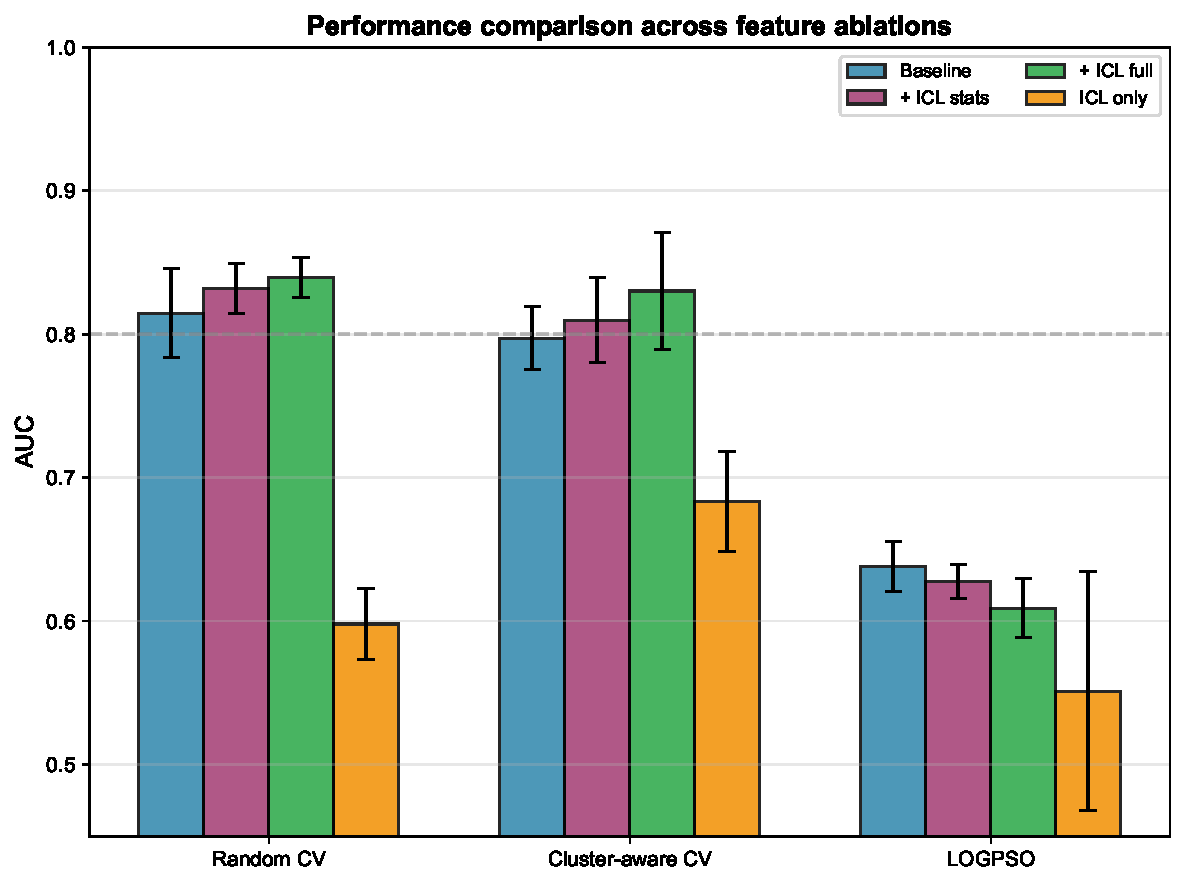
\includegraphics[width=0.9\textwidth]{../figures/figure1_performance_comparison.pdf}
\caption{Performance comparison across feature ablations under Random CV, Cluster-aware CV, and LOGPSO.}
\label{fig:perf_cmp}
\end{figure}

\subsection{Figure S2: ICL2/3 permutation importance}

\begin{figure}[H]
\centering
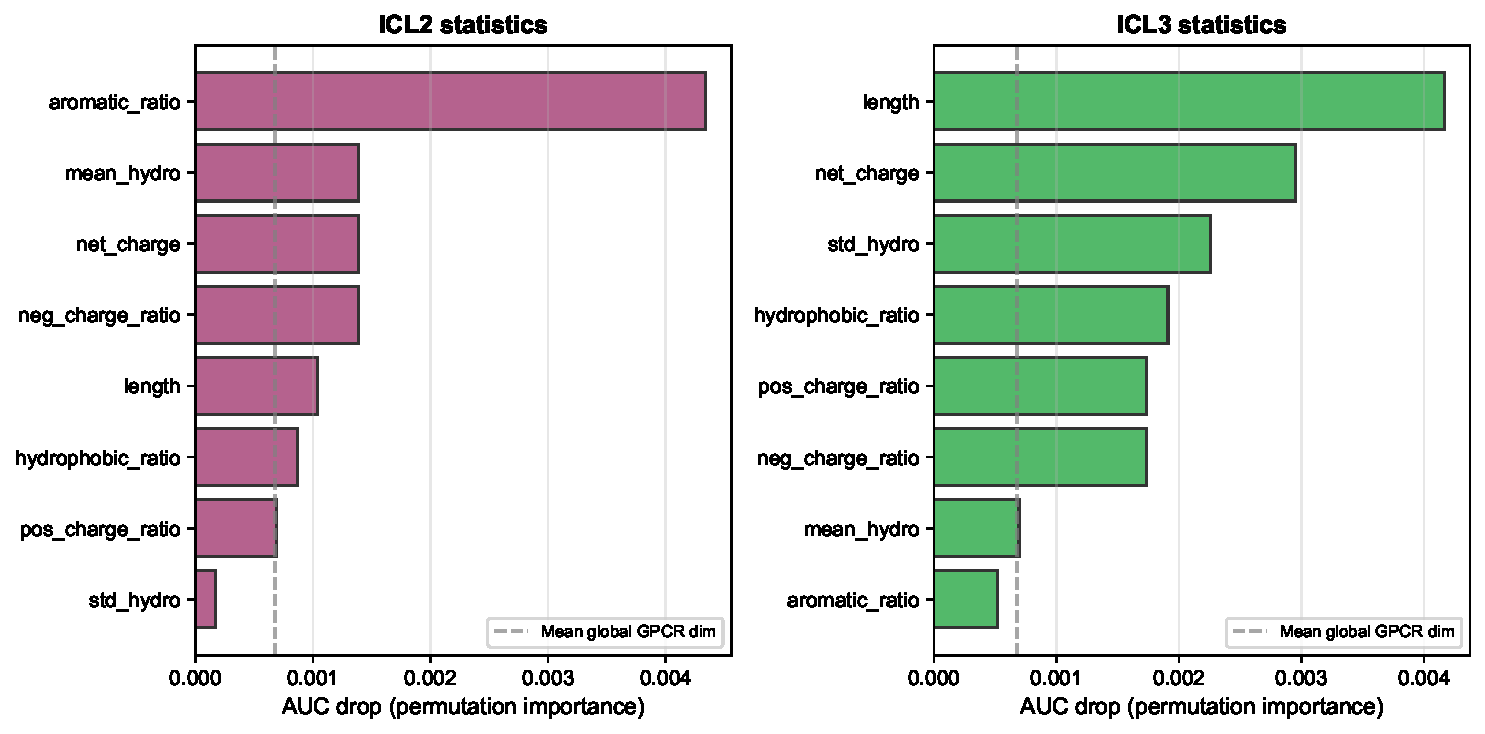
\includegraphics[width=0.95\textwidth]{../figures/figure2_icl_importance.pdf}
\caption{Permutation importance of ICL2 and ICL3 physicochemical statistics. The dashed line marks the mean importance of the 320 global GPCR ESM-2 dimensions.}
\label{fig:perm_imp}
\end{figure}

\subsection{Figure S3: SHAP residue-region mapping}

\begin{figure}[H]
\centering
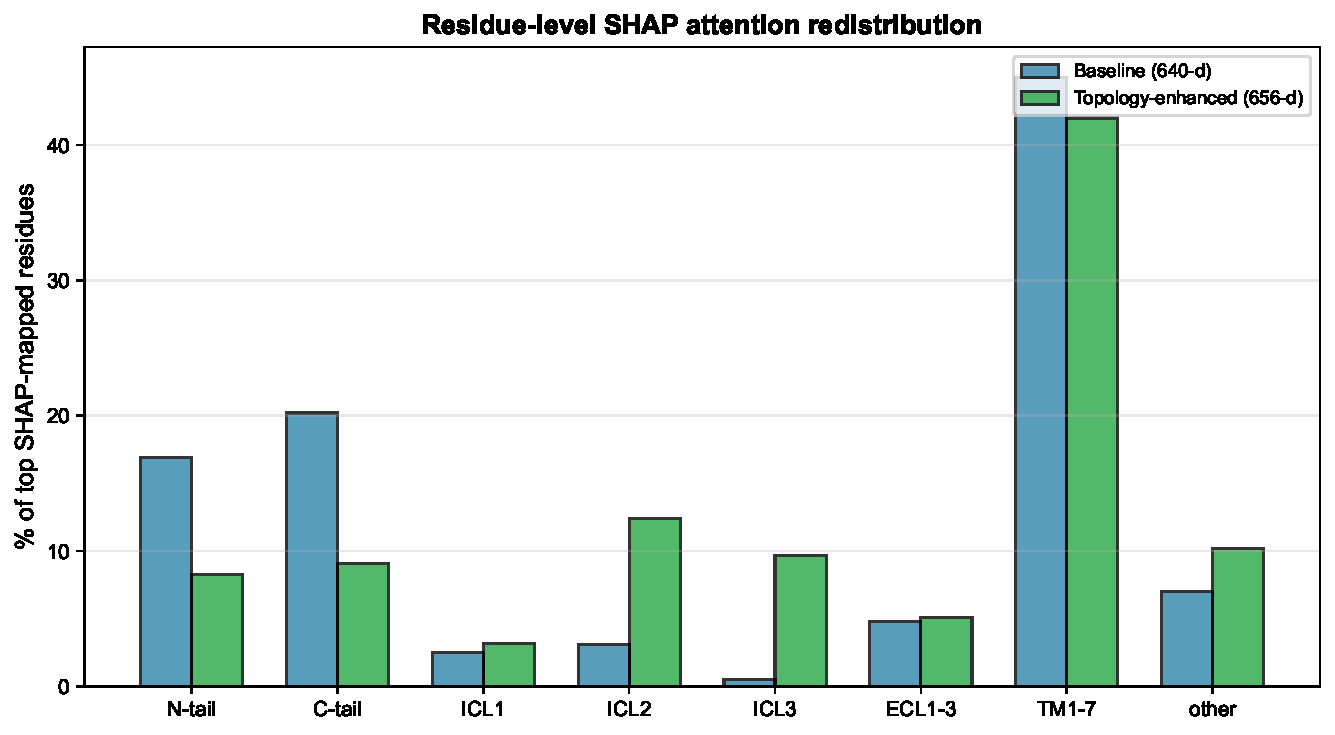
\includegraphics[width=0.85\textwidth]{../figures/figure3_shap_regions.pdf}
\caption{Residue-level SHAP weight redistribution from baseline (640-d) to topology-enhanced (656-d). After adding ICL features, model weight shifts from N-/C-tail regions toward the ICL2/3 interface.}
\label{fig:shap_map}
\end{figure}

\section{Code and Data Availability}

All source code, raw pairing matrices, cluster assignments, and evaluation scripts are available at \url{https://github.com/nblvguohao/topology-aware-gpcr-coupling}. The repository contains:
\begin{itemize}
    \item \texttt{extract\_esm\_features.py}: ESM-2 embedding extraction for protein sequences
    \item \texttt{fetch\_uniprot\_tm\_annotations.py}: batch-download UniProt TM annotations
    \item \texttt{extract\_icl\_features.py}: ICL2/3 loop extraction and feature computation
    \item \texttt{paired\_cross\_validation.py}: SVM baselines with Random/Cluster/LOGPSO CV
    \item \texttt{shap\_attribution.py}: SHAP-based feature-region importance analysis
    \item \texttt{permutation\_importance.py}: permutation importance of ICL2/3 statistics
    \item \texttt{generate\_figures.py}: publication-quality figure generation
\end{itemize}

\end{document}
